\documentclass{article}
\usepackage{amsmath}
\usepackage{mathtext}
\usepackage[T1,T2a]{fontenc}
\usepackage[utf8]{inputenc}
\usepackage[english, bulgarian, russian]{babel}
\usepackage{tikz}
\usepackage{pgfplots}
\usepackage[export]{adjustbox}
\usepackage[left=2cm,right=2cm,
    top=2cm,bottom=2cm,bindingoffset=0cm]{geometry}

\title{Измерение модуля Юнга методом акустического резонанса}
\date{2019-10-21}
\author{Панферов Андрей}

\begin{document}
\topmargin=-10mm
\pagenumbering{gooble}
\maketitle
\newpage
\pagenumbering{arabic}
Зависимость частоты от номера резонансного пика для трех измеряемых стержней занесем в Таблицу 1:
\begin{table}[h!]
\begin{center}
\caption{Резонансные частоты стержней}
\begin{tabular}{|c|c|c|c|c|c|c|c|c||c|}
\hline
 &n &1 &2 &3 &4 &5 &6 &7 &1/2 \\
\hline
 Медь& \textit{f}, кГц& 3.244& 6.460& 9.738& 12.979& 16.208& 19.446& 22.718& 1.622\\
\hline
 Сталь& \textit{f}, кГц& 4.122& 8.262& 12.373& 16.505& 20.617& 24.733& 28.837& \\
\hline
 Дюраль& \textit{f}, кГц& 4.253& 8.521& 12.763& 17.026& 21.260& 25.496& 29.724& \\
\hline
\end{tabular}
\end{center}
\end{table}

Построим графики зависимости \textit{f}(n):

\begin{tikzpicture}[scale = 1.8]
\begin{axis}[
    axis lines = left,
    legend style={at={(0.9, 0.3)}},
    xlabel = {n},
    ylabel = {\textit{f}, кГц},
    xmin=0, xmax=7,
    ymin=0, ymax=30,
	ymajorgrids = true,
	xmajorgrids = true
]
\addplot[
	mark = square, 
	mark options = {
		scale = 1.5, 
		fill = red, 
		draw = chucknorris
	},
	ymajorgrids = true,
	xmajorgrids = true,
	color = blue 
]  coordinates {
	(1, 3.244) (2, 6.460) (3, 9.738) (4, 12.979) (5, 16.208) (6, 19.446) (7, 22.718)};
\addplot[
	mark = triangle, 
	mark options = {
		scale = 1.5, 
		fill = blue, 
		draw = chucknorris
	},
	ymajorgrids = true,
	xmajorgrids = true,
	color = red
] coordinates {
	(1, 4.122) (2, 8.262) (3, 12.373) (4, 16.505) (5, 20.617) (6, 24.733) (7, 28.837)};
\addplot[
	mark = otimes, 
	mark options = {
		scale = 1.5, 
		fill = green, 
		draw = chucknorris
	},
	ymajorgrids = true,
	xmajorgrids = true,
	color = green
]  coordinates {
	(1, 4.253) (2, 8.521) (3, 12.763) (4, 17.026) (5, 21.260) (6, 25.496) (7, 29.724)};
\legend{ 
	Медь, 
	Сталь,
	Дюраль
};

\end{axis}
\end{tikzpicture}


Из графика методом наименьших квадратов получаем:
\begin{table}[h!]
\begin{center}
\caption{Скорости звука в стержнях}
\begin{tabular}{|c|c|c|c|c|}
\hline
 & $\textit{f}_1$, кГц& $\delta\textit{f}_1$, кГц& $c_{ст}$, м/c& $\delta c_{ст}$, м/c\\ 
\hline
 Медь& 3.245& $3 \cdot 10^{-3}$& 3894& 33\\
\hline 
 Сталь& 4.119& $2 \cdot 10^{-3}$& 4943& 35\\
\hline 
 Дюраль& 4.245& $3 \cdot 10^{-3}$& 5094& 36\\
\hline 
\end{tabular}
\end{center}
\end{table}

\newpage

\begin{table}[h!]
\centering
\begin{minipage}[h]{0.30\linewidth}
\centering
Измерим линейные размеры и массу образцов из меди, стали и дюраля. Данные занесем в таблицу 2. Вычислим плотность материалов.
\end{minipage}
\begin{minipage}[h]{0.2\linewidth}
\centeging
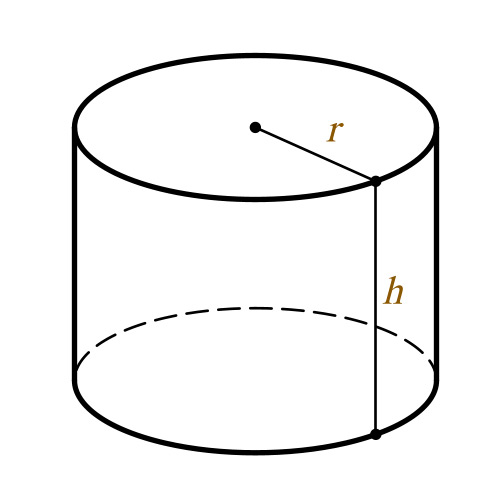
\includegraphics[width=1\textwidth]{cyl.jpg}
\end{minipage}
\begin{minipage}[h]{0.54\linewidth}
\centering

\begin{tabular}{|c|c|c|c|c|c|}
\hline
 & \textit{m}, г& h, мм& 2r, мм& $\rho$, $кг/м^3$& $\delta\rho$, $кг/м^3$\\
\hline
Медь & 41.370& 41.5& 11.95& $8.89 \cdot 10^3$& $ 3 \cdot 10^1$\\
\hline
Сталь & 35.206& 40.0& 11.99& $7.80 \cdot 10^3$& $ 3 \cdot 10^1$\\
\hline
Дюраль & 9.201& 30.0& 11.84& $2.79 \cdot 10^3$& $ 1.1 \cdot 10^1$\\
\hline
\end{tabular}
\label{table2}
\caption{Параметры образцов}
\end{minipage}
\end{table}

\begin{equation*}
\end{equation*}

Измерим среднее значение диаметров стрежней d=2R:
\begin{table}[h!]
\begin{center}
\caption{Диаметры исследуемых стержней (в мм)}
\begin{tabular}{|c|c|c|c|c|c|c|c|c|c|c|}
\hline
 Медь& 11.96& 11.95& 11.96& 11.96& 11.96& 11.95& 11.96& 11.96\\
\hline
 Сталь& 11.72& 12.11& 12.04& 11.94& 12.33& 11.86& 12.10& 11.87\\
\hline
 Дюраль& 11.72& 11.73& 11.74& 11.75& 11.76& 11.75& 11.75& 11.76\\
\hline
\end{tabular}
\end{center}
\end{table}

Как мы видим, $R/\lambda \approx R/L \approx 10^{-2}$, что сравнимо с приборной погрешностью измерений

\begin{equation*}
\end{equation*}

\begin{center}
\caption{\textbf{Финальные результаты}
\end{center}

\begin{center}
Вычислим и занесем в Таблицу 5 модули Юнга материалов:
\end{center}
\begin{table}[h!]
\begin{minipage}[h]{0.6\linewidth}
\begin{tabular}{|c|c|c|c|c|}
\hline
 & E, ГПа& $\delta$E, ГПа& $E_{тб}, ГПа& $|E_{тб}-E|$, ГПа\\
\hline
 Медь& 135 & 3& 110& 25\\
\hline
 Сталь& 191& 3&  ?& ?\\
\hline
 Дюраль& 72& 1.1& 74& 2\\
\hline
\end{tabular}
\caption{Модули Юнга}
\end{minipage}
\begin{minipage}[h]{0.3\linewidth}
\begin{align*}
E =& c_{ст}^2 \cdot \rho& \\
\delta E =& \sqrt{4(\frac{\delta c_{ст}}{c_{ст}})^2 + (\frac{\delta\rho}{\rho})^2}&
\end{align*}
\end{minipage}
\end{table}

\begin{equation*}
\end{equation*}

Вывод: метод акустического резонанса является точным и надежным методом измерения модуля Юнга металлов.

\newpage

\begin{center}
\textbf{Задание 12*}
\end{center}

\begin{minipage}[h]{0.44\linewidth}
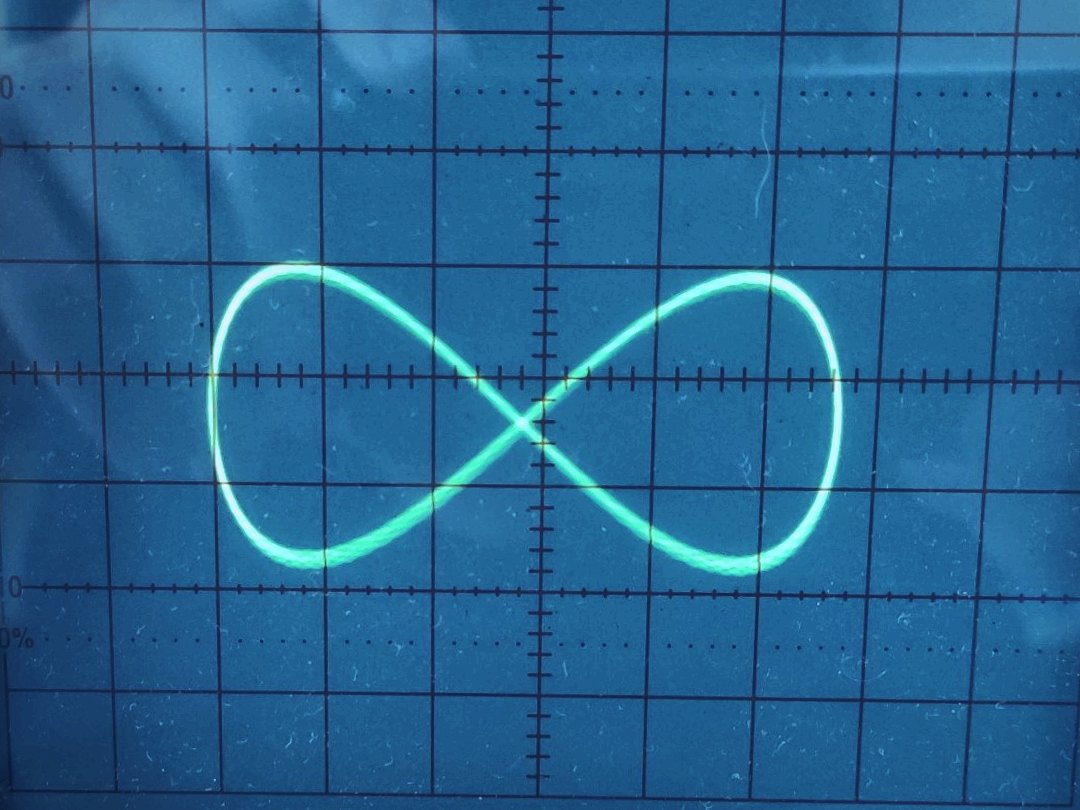
\includegraphics[width=1\textwidth]{screen.jpg}
\end{minipage}
\begin{minipage}[h]{0.10\linewidth}
\end{minipage}
\begin{minipage}[h]{0.44\linewidth}
Как мывидим, модуляция на частоте $\textit{f}_1/2$ вызывает колебания на частоте $\textit{f}_1$
\end{minipage}

\begin{equation*}
\end{equation*}

\begin{center}
\textbf{Задание 13*}
\end{center}

\begin{table}[h!]
\begin{minipage}[h]{0.3\linewidth}
\centered
\begin{tabular}{|c|c|c|c|}
\hline
 $U_{in}$, дел& U_{out}, дел& \textit{f}, кГц& \textit{f}, кГц\\
 \hline
 4.0& 2.0& 4.2490& 4.2542\\
 \hline
 4.0& 2.4& 4.2498& 4.2538\\
 \hline
 4.0& 2.8& 4.2504& 4.2536\\
 \hline
 4.0& 3.2& 4.2506& 4.2534\\
 \hline
 4.0& 3.6& 4.2508& 4.2532\\
 \hline
 4.0& 4.0& 4.2510& 4.2530\\
 \hline
 4.0& 4.4& 4.2512& 4.2529\\
 \hline
 4.0& 4.8& 4.2512& 4.2528\\
 \hline
 4.0& 5.2& 4.2515& 4.2527\\
 \hline
 4.0& 5.6& 4.2515& 4.2526\\
 \hline
 4.0& 6.0& 4.2516& 4.2525\\
 \hline
 4.0& 6.4& 4.2518& 4.2523\\
 \hline
 4.0& 6.8& 4.2521& 4.25\\
 \hline
\end{tabular}
\caption{АЧХ}
\end{minipage}
\begin{minipage}[h]{0.69\linewidth}

\begin{tikzpicture}[scale = 1.3]
\begin{axis}[
    axis lines = left,
    xlabel = {\textit{f}, кГц},
    ylabel = {$U_{out}$, В},
    xmin=4.2490, xmax=4.2550,
    ymin=1.8, ymax=7,
	ymajorgrids = true,
	xmajorgrids = true
]
\addplot[
	mark = square, 
	mark options = {
		scale = 1.5, 
		fill = red, 
		draw = chucknorris
	},
	ymajorgrids = true,
	xmajorgrids = true,
	color = red 
]  coordinates {(4.2490,2.0)(4.2498,2.4)(4.2504,2.8)(4.2506,3.2)(4.2508,3.6)(4.2510,4.0)(4.2512,4.4)(4.2513,4.8)(4.2513,5.2)(4.2515,5.6)(4.2516,6.0)(4.2518,6.4)(4.2521,6.8)(4.2523,6.4)(4.2525,6.0)(4.2526,5.6)(4.2527,5.2)(4.2528,4.8)(4.2529,4.4)(4.2530,4.0)(4.2532,3.6)(4.2534,3.2)(4.2536,2.8)(4.2538,2.4)(4.2542,2.0)
	};

\end{axis}
\end{tikzpicture}

\end{minipage}
\end{table}

\begin{equation*}
\end{equation*}

\begin{minipage}[t]{0.33\linewidth}
\centered
\begin{equation*}
\delta\textit{f} = (0.015 \pm 2) \: кГц
\end{equation*}
\end{minipage}
\begin{minipage}[t]{0.33\linewidth}
\centered
\begin{equation*}
\textit{f} = (4.2521 \pm 0.0002) \: кГц
\end{equation*}
\end{minipage}
\begin{minipage}[t]{0.33\linewidth}
\centered
\begin{equation*}
\sigma = \frac{\textit{f}}{\delta\textit{f}} = (2.8 \pm 0.4) \cdot 10^{3}
\end{equation*}
\end{minipage}
\begin{minipage}[h]{0.25\linewidth}
\centered
\begin{equation*}
\end{equation*}
\end{minipage}

\end{document}

